%!TEX root = latex/refman.tex

\chapter{Introdução}

Ao se utilizar programação para resolver problemas científicos, a escolha da estrutura de dado correta para representar os dados pode acarretar em diferenças consideráveis no tempo de execução e consumo de memória do programa. Este trabalho apresenta uma implementação em C++ de duas das principais estruturas de dados utilizadas em sistemas computacionais, a pilha e a fila, ambas utilizando listas duplamente encadeadas como representação principal.

O programa foi implementado utilizando orientação a objetos, sendo que todas as estruturas foram criadas em classes separadas. Também foi feito o uso de \emph{templates} em C++ para possibilitar o armazenamento de qualquer tipo de objeto nos nós da estrutura.

\section{Objetivo}

Implementar uma pilha e uma fila na linguagem C++ utilizando orientação a objetos e vetores primitivos como método de armazenamento de dados interno.

Implementar uma pilha e uma fila na linguagem C++ utilizando alocação dinâmica de memória, herança e polimorfismo. A herança deve ser feita de uma lista encadeada.

\chapter{Referencial Teórico}

A pilha é uma estrutura de dados do tipo \emph{last in, first out} (LIFO), ou seja, em uma pilha, o último objeto a ser inserido é o primeiro a ser removido. Na pilha, as operações de inserção e remoção são feitas com complexidade \(O(1)\) \cite{cormen_introduction_2009}, utilizando-se uma referência para o topo da pilha. A operação de consulta retorna o último valor inserido na pilha sem removê-lo, também em \(O(1)\).

A fila é uma estrutura de dados do tipo \emph{first in, first out}, ou seja, elementos inseridos primeiro são os primeiros a serem removidos. Na fila, são mantidas referências ao primeiro e ao último elemento, permitindo que operações de inserção no fim da estrutura sejam feitas com complexidade \(O(1)\) e que remoções no início da estrutura também tenham complexidade \(O(1)\) \cite{cormen_introduction_2009}. A consulta ao primeiro elemento da fila também é feita em \(O(1)\).

Tanto a pilha como a filha não prevêm operações de busca ou navegação.

Existem duas formas canônicas de se implementar estas estruturas de dados. A primeira consiste na utilização de um vetor de tamanho estático pré-definido para o armazenamento dos dados da estrutura. A figura \ref{fig:stack} exibe uma pilha \(S\) implementada com um vetor de \(7\) posições. O atributo \(top\) mantém a posição do topo da pilha, isto é, a posição no vetor do último valor inserido na pilha (\ref{fig:stack1}). Na figura \ref{fig:stack2}, dois novos valores são inseridos na pilha, aumentando o valor de \(top\) em \(2\). Por último, na figura \ref{fig:stack3}, o último valor que havia sido inserido na pilha é removido.

\begin{figure}
  \centering
  \subfloat[]{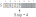
\includegraphics[width=.3\linewidth]{../static_stack1}\label{fig:stack1}}

  \subfloat[]{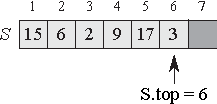
\includegraphics[width=.3\linewidth]{../static_stack2}\label{fig:stack2}}

  \subfloat[]{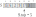
\includegraphics[width=.3\linewidth]{../static_stack3}\label{fig:stack3}}
  \caption{Fonte: ``adaptado de'' \cite{cormen_introduction_2009}}.\label{fig:stack}
\end{figure}

A figura \ref{fig:queue} apresenta uma fila circular \cite{cormen_introduction_2009} implementada utilizando um vetor de 12 posições. Na fila circular, variáveis mantêm a posição do início e fim da fila (\(head\) e \(tail\), respectivamente). Em um vetor com índices iniciados em 0, quando um elemento é removido da fila, \(head \leftarrow (head - 1) \bmod n\). Igualmente, ao inserir um item na fila circular, \(tail \leftarrow (tail + 1) \bmod n\). Para saber quando a pilha está cheia ou vazia, é possível manter um contador.

A figura \ref{fig:queue1} apresenta uma fila circular implementada com um vetor de tamanho 12, iniciando em \(head = 7\) e terminando em \(tail = 12\). Na figura \ref{fig:queue2}, três novos valores são inseridos e \(tail\) passa do fim para o início da fila. Em \ref{fig:queue3}, um elemento é removido da fila e o valor de \(head\) é incrementado. O valor não precisa ser apagado do vetor e será sobrescrito se necessário.

\begin{figure}
  \centering
  \subfloat[]{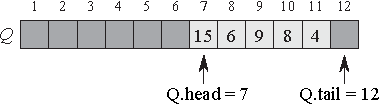
\includegraphics[width=.5\linewidth]{../circular_buffer1}\label{fig:queue1}}

  \subfloat[]{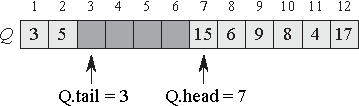
\includegraphics[width=.5\linewidth]{../circular_buffer2}\label{fig:queue2}}

  \subfloat[]{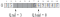
\includegraphics[width=.5\linewidth]{../circular_buffer3}\label{fig:queue3}}
  \caption{Fonte: ``adaptado de'' \cite{cormen_introduction_2009}}.\label{fig:queue}
\end{figure}

\section{Lista encadeada}

A segunda forma de se implementar essas estruturas involve o uso de alocação dinâmica de memória e uma lista encadeada para se armazenar os dados. Nesta abordagem, o tamanho máximo tanto das estruturas (tanto pilha, como fila ou lista) não precisa ser pré-definido.

De acordo com \cite{cormen_introduction_2009}, uma lista é uma estrutura que ordena dados de maneira linear. Assim como a pilha e fila de tamanho estático, uma lista também pode ser implementada em C++ através de um vetor primitivo de dados. Uma lista encadeada se diferencia ao criar nós que, além de armazenarem dados, são capazes de referenciar um nó adicional. Quando cada nó referencia um nó com o próximo elemento inserido, a linearidade é garantida e uma lista encadeada é criada. O encadeamento permite que a estrutura seja criada sem um tamanho pré-determinado, possibilitando que ela cresça conforme necessário e economize memória ao diminuir, caso seus dados sejam devidamente destruídos.

Em uma lista duplamente encadeada, cada nó armazena, adicionalmente, uma referência ao elemento anterior, permitindo que a estrutura seja navegada em ambas as direções.

A figura \ref{fig:list} demonstra as funcionalidades de uma lista duplamente encadeada \(L\). Em \ref{fig:list1}, quatro valores são mantidos inicialmente em \(L\), assim como uma referência ao início e fim da lista em \(L.head\) e \(L.tail\), respectivamente. Em \ref{fig:list2}, um valor adicional é inserido no início de \(L\) e a referência de \(\L.head\) é atualizada para o novo valor. Por último, em \ref{fig:list3}, o valor na quarta posição de \(L\) é removido e as conexões entre o terceiro e quinto elemento são atualizadas.

\begin{figure}[h!]
  \centering
  \subfloat[]{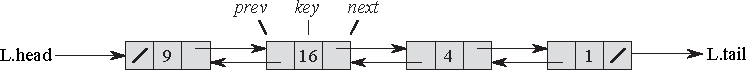
\includegraphics[width=.8\linewidth]{../doubly_linked_list1}\label{fig:list1}}

  \subfloat[]{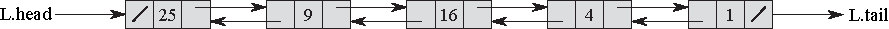
\includegraphics[width=.8\linewidth]{../doubly_linked_list2}\label{fig:list2}}

  \subfloat[]{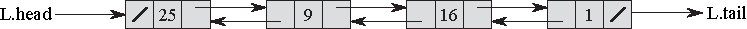
\includegraphics[width=.8\linewidth]{../doubly_linked_list3}\label{fig:list3}}
  \caption{Fonte: ``adaptado de'' \cite{cormen_introduction_2009}}.\label{fig:list}
\end{figure}

De acordo com \cite{cormen_introduction_2009} as operações de inserção e remoção em uma lista possuem complexidade \(O(1)\), contanto que seja passada uma referência direta ao local na estrutura onde se deseja realizar a operação. A operação de busca possui complexidade \(O(n)\), uma vez que, no pior caso, toda a estrutura deve ser vasculhada. O uso de listas encadeadas como representação para pilhas e filas é possível uma vez que, na lista, inserções e remoções no início e no fim da estrutura podem ser feitas com complexidade \(O(1)\), dado que referências ao primeiro e último elementos da lista sejam mantidas. Esta abordagem de implementação, apresentada em \cite{deitel_cpp_2012}, é utilizada aqui.

\section{Lista ordenada}

A lista ordenada é uma lista encadeada na qual a posição em que um elemento é inserido depende de algum tipo de ordenação. Para tanto, toda vez que um novo elemento é inserido, ele é comparado a todos os outros elementos da lista até que sua posição seja encontrada.

\chapter{Implementação}

A implementação das estruturas de dados se utilizou da orientação a objetos para organizar as estruturas em classes; herança, que possibilitou a reutilização de código entre estruturas semelhantes, assim como o compartilhamento da documentação dos métodos herdados; polimorfismo, permitindo que estruturas de uma mesma super-classe (\emph{e.g.} todas as pilhas que herdam de uma mesma super-classe) fossem testadas usando a mesma função de testes; \emph{templates}, que permitem que o tipo de dado a ser armazenado pela estrutura de dados seja escolhido quando o objeto que representa a estrutura é criado; e, por último, exceções, tratando casos especiais como \emph{underflow}, \emph{overflow} e busca por índices inexistentes.

Classes e métodos foram documentados utilizando o padrão de comentários exigido pelo software Doxygen, o qual se responsabiliza pela geração da documentação em formato \LaTeX{}, HTML ou RTF.

Foram implementadas as seguintes classes concretas:

\begin{description}
  \item[StaticStack:] pilha estática utilizando vetores primitivos como armazenamento de dados;
    \item[StaticQueue:] fila estática utilizando vetores primitivos como armazenamento de dados;
      \item[DynamicStack:] pilha dinâmica, utiliza alocação dinâmica de memória;
        \item[DynamicQueue:] fila dinâmica, utiliza alocação dinâmica de memória;
          \item[LinkedList:] lista duplamente encadeada;
            \item[OrderedList:] lista ordenada duplamente encadeada;
            \item[Node:] nó utilizado na estruturas dinâmicas.
\end{description}

Foram implementadas as seguintes classes abstratas:

\begin{description}
  \item[DataStructure:] super-classe de todas as estruturas, contém funções pertinentes a todas elas;
  \item[Stack:] super-classe de \emph{StaticStack} e \emph{DynamicStack};
  \item[Queue:] super-classe de \emph{StaticQueue} e \emph{DynamicQueue}.
\end{description}

Por último, a classe \textbf{ProtectedLinkedList} é utilizada nas implementações de \emph{DynamicStack} e \emph{DynamicQueue}, escondendo métodos característicos de uma lista encadeada, porém inexistentes em pilhas e filas, como inserção em pontos intermediários da estrutura e busca por elementos. Esses métodos são expostos através da classe \emph{LinkedList}, compondo uma estrutura de dados completa e individual.
